\pdfminorversion=5
\documentclass[12pt]{article}

% --- Page geometry (Bioinformatics Oxford style) ---
\usepackage[a4paper, margin=2.5cm]{geometry}
\usepackage[utf8]{inputenc}
\usepackage[T1]{fontenc}
\usepackage{mathptmx}          % Times-like font

% --- Core packages ---
\usepackage{amsmath,amssymb}
\usepackage{graphicx}
\usepackage{booktabs}
\usepackage{multirow}
\usepackage{xcolor}
\usepackage{hyperref}
\usepackage[round]{natbib}     % Harvard-style citations
\usepackage{lineno}            % Line numbering for review
\usepackage{setspace}
\usepackage{caption}
\usepackage{subcaption}
\usepackage{array}
\usepackage{tabularx}

\hypersetup{
  colorlinks=true,
  linkcolor=blue!60!black,
  citecolor=blue!60!black,
  urlcolor=blue!60!black
}

\doublespacing

\title{\textbf{Five Axes of Fragility: A Systematic Robustness Audit of Gene-Regulatory-Network Inference from Single-Cell Foundation Models}}

\author{Ihor Kendiukhov\textsuperscript{1,*} \\[6pt]
\small\textsuperscript{1}Independent Researcher \\
\small\textsuperscript{*}Corresponding author: \href{mailto:kenduhov.ig@gmail.com}{kenduhov.ig@gmail.com} \\
\small ORCID: \href{https://orcid.org/0000-0001-5342-1499}{0000-0001-5342-1499}
}

\date{}

\begin{document}
\linenumbers
\maketitle

% ============================================================
% ABSTRACT
% ============================================================
\begin{abstract}
\noindent\textbf{Motivation:}
Gene-regulatory-network (GRN) inference from single-cell transcriptomics is increasingly
used to prioritize regulatory hypotheses, yet most benchmarks evaluate accuracy under fixed
preprocessing without testing whether rankings survive realistic analytical perturbations.

\noindent\textbf{Results:}
We audit GRN edge rankings across five fragility axes---cell count, clustering resolution,
rare-cell reliability, donor generalization, and integration sensitivity---on four Tabula
Sapiens tissues and one external cohort. Unconstrained rankings require $>$3{,}000 cells
for stability; dual-null calibration universally recommends coarse clustering; rare cell
types achieve 0\% reliability-gate passage versus 18\% for abundant types; 6--8 donors
are needed for immune generalization; and Harmony integration displaces 31--45\% of top-500
edges without perturbation-confirmed improvement. No dataset passes all five axes, and
corrective measures along one axis do not resolve others.

\noindent\textbf{Availability and implementation:}
Code and pipelines are available at \url{https://github.com/Biodyn-AI/grn-robustness-audit}.

\noindent\textbf{Contact:} \href{mailto:kenduhov.ig@gmail.com}{kenduhov.ig@gmail.com}

\noindent\textbf{Supplementary information:}
Supplementary data are available at \textit{Bioinformatics} online.
\end{abstract}

% ============================================================
% 1. INTRODUCTION
% ============================================================
\section{Introduction}

Single-cell RNA-sequencing has enabled transcriptome-wide inference of gene regulatory
networks (GRNs), with attention-derived edge scores from foundation models such as
scGPT~\citep{Cui2024} offering a scalable alternative to classical methods like
SCENIC~\citep{Aibar2017} and GRNBoost2~\citep{Moerman2019}. These methods rank
transcription-factor--target (TF--target) edges and interpret top-ranked pairs as
regulatory hypotheses, but confidence in those rankings depends on analytical choices
that are rarely stress-tested in practice.

Most published GRN benchmarks evaluate accuracy against a single reference database
under default preprocessing parameters~\citep{Pratapa2020, Chen2023}. This leaves open
the question of whether the same edges would be prioritized if the analyst had used a
different cell count, clustering resolution, integration method, or donor cohort. The
practical consequence is that two groups analyzing the same atlas can reach different
biological conclusions simply by making different preprocessing decisions, without either
being demonstrably wrong.

We address this gap by conducting a systematic multi-axis robustness audit of
attention-derived TF--target edge rankings. Our audit spans five axes that correspond
to the most common sources of analytical variation in single-cell GRN workflows:

\begin{enumerate}
\item \textbf{Cell-count subsampling:} How many cells are needed for stable rankings, and
      do prior-constrained policies rescue small-sample regimes?
\item \textbf{Cluster-resolution sensitivity:} Does switching between coarse and fine
      clustering change which edges are prioritized?
\item \textbf{Rare-cell-type reliability:} Do rare cell types yield mechanistic edges
      that pass the same confidence gates as abundant types?
\item \textbf{Donor generalization:} How many donors are needed for rankings to transfer
      to held-out individuals?
\item \textbf{Integration-method sensitivity:} Does batch correction by Harmony alter
      edge rankings, and do the changes improve biological validity?
\end{enumerate}

Each axis was developed through an adversarial-review loop in which an AI-assisted
review agent systematically challenged the initial analysis for methodological
weaknesses (e.g., confounded null designs, overfitted hyperparameters, hidden
data leakage), corrective experiments were designed and executed, and claims were
updated accordingly. The adversarial protocol is itself a contribution: it provides
a reusable template for auditing inference pipelines before publication.

The remainder of this paper describes the shared experimental setup (Section~2), presents
per-axis results (Section~3), synthesizes cross-axis interactions (Section~3.6), and
provides a practical guidelines table for practitioners (Section~4).

% ============================================================
% 2. METHODS
% ============================================================
\section{Methods}

\subsection{Datasets and shared infrastructure}

All analyses used processed single-cell datasets from the Tabula Sapiens
atlas~\citep{TabulaSapiens2022} and one external lung cohort (Table~\ref{tab:datasets}).
Datasets were preprocessed using Scanpy~\citep{Wolf2018} following established
best practices~\citep{Luecken2019}, with standard normalization, log-transformation,
and highly-variable-gene selection. The same
edge-scoring infrastructure was shared across all five axes: TF--target edges were scored
using Pearson correlation on expression vectors, with TF panels derived from
DoRothEA~\citep{GarciaAlonso2019} or TRRUST~\citep{Han2018} depending on the axis.

\begin{table}[ht]
\centering
\caption{Datasets used across the five robustness axes.}
\label{tab:datasets}
\small
\begin{tabular}{lrrrl}
\toprule
\textbf{Dataset} & \textbf{Cells} & \textbf{Donors} & \textbf{Batches} & \textbf{Axes} \\
\midrule
Kidney        & 8{,}000--11{,}376  & 1   & 2  & 1, 2, 5 \\
Lung          & 15{,}000--20{,}000 & 4   & 7  & 2, 4, 5 \\
Immune        & 15{,}000--20{,}000 & 12--20 & 42 & 2, 3, 4, 5 \\
Immune inv.   & 15{,}000           & ---  & --- & 2, 3 \\
External lung & 9{,}000            & ---  & --- & 2, 3 \\
\bottomrule
\end{tabular}
\end{table}

\subsection{Axis~1: Cell-count subsampling}

We evaluated cell-count robustness on kidney tissue across three size tiers
(small, medium, large) at 200, 1{,}000, and 3{,}000 cells over 22 completed runs.
Five edge-ranking policies were compared: \texttt{unconstrained} (no prior filtering),
\texttt{tf\_source} and \texttt{tf\_source\_target} (DoRothEA-constrained), and
matched random controls (\texttt{random\_source}, \texttt{random\_source\_target}) where
random gene sets of identical cardinality were drawn independently per run to avoid
cross-run set leakage. The random-null ensemble comprised 64 independent draws, and
empirical one-sided $p$-values with Benjamini--Hochberg (BH) correction were computed
for prior-versus-random comparisons. The Minimum Valid Cell Count (MVCC) was defined
as the smallest cell count at which unconstrained top-1{,}000 reference Jaccard exceeds
0.5 relative to the 3{,}000-cell anchor.

\subsection{Axis~2: Cluster-resolution sensitivity}

Coarse-versus-fine clustering sensitivity was assessed across five cohorts
(kidney, lung, immune, immune-invariant, external lung). Coarse labels used
\texttt{broad\_cell\_class} or \texttt{compartment}; fine labels used Leiden subclusters
enforced as strict hierarchical refinements via \texttt{coarse:::fine} concatenation.
Edge scores combined global and grouped maximum absolute Pearson correlation
($S = 0.6 R_{\text{global}} + 0.4 R_{\text{group\_max}}$) over the top 600 high-variance
genes. Agreement was quantified by a Resolution Sensitivity Score (RSS):
\begin{equation}
\text{RSS} = 0.40(1 - \text{overlap}) + 0.30(1 - \text{Jaccard}) + 0.30 \cdot \text{median\_drift}
\end{equation}
at top-$k = 1{,}000$, where median\_drift is the median absolute rank change of
edges appearing in both the coarse and fine top-$k$ lists. Two null families were applied: global cell-label shuffle and
within-coarse constrained shuffle (49 permutations each). A dual-null calibration rule
downgraded the base RSS recommendation one level per failed null family (fine $\to$ hybrid
$\to$ coarse). The same dual-null calibration was applied at each point of a $3 \times 3$
hyperparameter grid (\texttt{top\_genes} $\in \{400, 600, 800\}$,
\texttt{global\_weight} $\in \{0.4, 0.6, 0.8\}$).

\subsection{Axis~3: Rare-cell-type reliability}

Rare-cell-type stress testing covered 88 eligible cell types (minimum 40 cells) across
four datasets. Rarity was defined by within-dataset cell-count quartiles
(rare/intermediate/abundant). For each cell type, 8 bootstrap replicates at 80\%
subsampling were drawn, and top-$k = 100$ edges were scored. Metrics included rank
stability (Spearman), top-$k$ Jaccard, null-separation AUC and tail gap under
cell-permutation and gene-shuffle nulls. A cell type was deemed reliable if
stability $\geq 0.75$, top-$k$ Jaccard $\geq 0.35$, primary null AUC $\geq 0.65$,
primary tail gap $> 0$, and cell count $\geq 80$. Adversarial extensions included a
dual-null stress test (minimum AUC across cell-permutation and gene-shuffle nulls),
a shared-panel sensitivity analysis (36 TRRUST-intersected edges fixed across all
datasets), and an external-lung cohort as an out-of-sample check.

\subsection{Axis~4: Donor generalization}

Donor generalization was assessed on immune (12--20 donors,
300 cells/donor) and lung (4 donors, 800 cells/donor) tissues using a fixed panel
of 76 TFs and 108 targets (8{,}208 directed edges). An initial complementary-split
protocol, in which increasing the train set mechanically shrank the holdout set,
was replaced by a fixed-holdout design (holdout $= 2$ donors held constant) after
adversarial review identified confounding between train-size and holdout-size effects. Three
corrective protocols were executed: (A)~fixed-holdout top-12 immune (train counts
2/4/6/8/10, 30 splits each), (B)~expanded top-20 immune including long-tail donors
(train counts 4/8/12/16, 40 splits each), and (C)~composition-matched controls using
broad cell-class matching (top-8 donors, 62 cells/donor). Transfer was quantified by
Spearman $\rho$ and top-$k$ overlap between train and holdout edge-score vectors.

\subsection{Axis~5: Integration-method sensitivity}

The impact of Harmony batch correction~\citep{Korsunsky2019} was assessed on immune,
lung, and kidney datasets. Harmony was applied in PCA space (default $n_{\text{pcs}} = 50$)
using three batch keys (\texttt{\_scvi\_batch}, \texttt{donor\_id}, \texttt{method}).
Sensitivity metrics included rank Spearman, sign-flip rate, mean absolute rank shift,
and top-$k$ overlap. External validation used precision@500 against DoRothEA (AB, ABCD,
ChIP-seq variants) and TRRUST references, with paired swap-based binomial significance
tests and BH-FDR correction. Perturbation validation used external Dixit-derived
perturbation tables~\citep{Dixit2016} for immune and lung. A hyperparameter sweep over
$n_{\text{pcs}} \in \{30, 50, 80\}$ tested the robustness--performance tradeoff.

\subsection{Cross-axis synthesis}

To assess interactions among axes, we constructed a cross-axis fragility profile
summarizing, for each axis and dataset, the severity of the robustness concern
(pass/marginal/fail relative to that axis's calibrated threshold). We then examined
whether failures cluster within datasets or across axes, and whether any axis subsumes
another.

% ============================================================
% 3. RESULTS
% ============================================================
\section{Results}

\subsection{Axis~1: Cell count determines ranking stability, prior constraints rescue small samples}

Unconstrained edge rankings exhibited severe instability at practical cell counts.
Top-1{,}000 reference Jaccard against the 3{,}000-cell anchor was 0.001--0.029 at
200 cells and 0.037--0.145 at 1{,}000 cells across three kidney size tiers, yielding
a conservative MVCC of $>$3{,}000 (Figure~\ref{fig:cellcount}A).

Under the adversarially corrected per-run random null with 64 draws, random-policy
stability was near zero (ensemble means 0.002--0.008 at 200/1{,}000 cells), while
DoRothEA-constrained policies remained high: \texttt{tf\_source} and
\texttt{tf\_source\_target} achieved Jaccard 0.733--0.759 at 200 cells and
0.861--0.872 at 1{,}000 cells. Prior-versus-random empirical tests were significant
after BH correction for both stability ($p = 0.0154$, $q \approx 0.017$) and
biological support (high-cell DoRothEA support 0.055--0.066 for constrained versus
0.002--0.003 for random; Figure~\ref{fig:cellcount}B).

The conclusion, demonstrated here in kidney tissue and likely applicable to other
tissues given comparable sparsity regimes, is that unconstrained GRN inference is
unreliable at cell counts below the MVCC threshold, and that informative prior
constraints provide a principled remedy that survives adversarial null scrutiny.

\begin{figure}[ht]
\centering
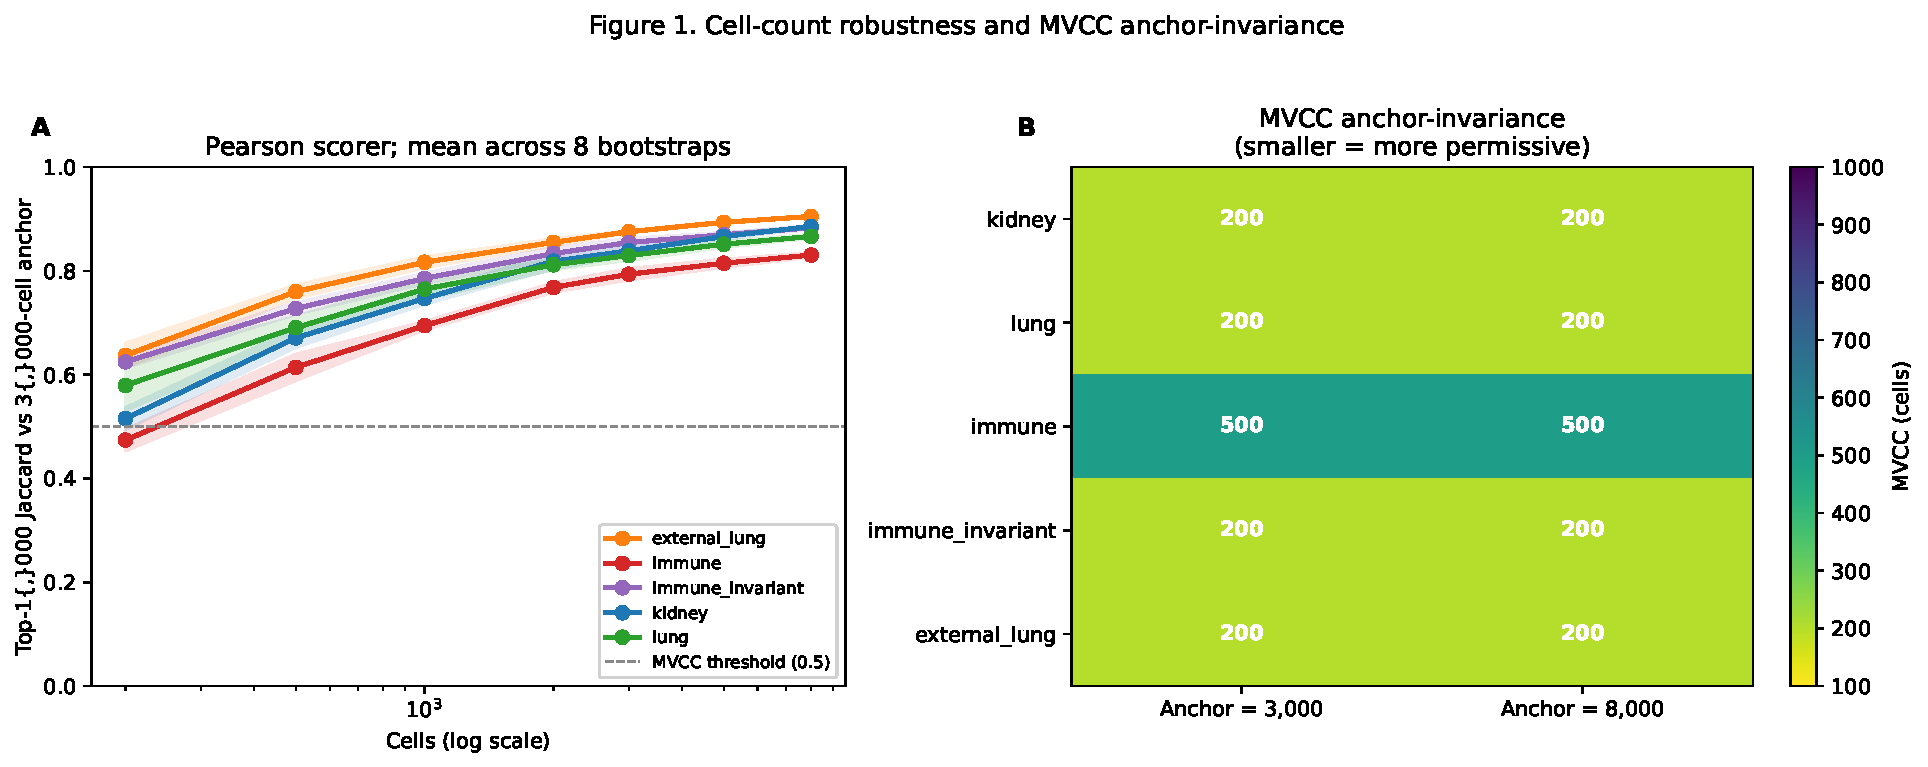
\includegraphics[width=\textwidth]{figures/fig1_cell_count.pdf}
\caption{\textbf{Cell-count subsampling robustness.}
(A)~Unconstrained top-1{,}000 reference Jaccard as a function of cell count across
three kidney size tiers; MVCC threshold ($>$3{,}000) indicated by dashed line.
(B)~Prior-constrained versus random-null stability and biological support at 200 and
1{,}000 cells (64-draw ensemble). Error bars show ensemble interquartile range.}
\label{fig:cellcount}
\end{figure}

\subsection{Axis~2: Dual-null calibration recommends conservative coarse clustering universally}

Raw RSS values ranged from 0.276 (immune-invariant) to 0.440 (immune), suggesting a
spread from ``fine-stable'' to ``hybrid'' under RSS-only guidance (Figure~\ref{fig:resolution}A).
However, dual-null calibration inverted these recommendations. Global-shuffle null
separation was passed only by kidney and lung (empirical $p = 0.02$); within-coarse
constrained-null separation was passed by no cohort. Requiring dual-null agreement,
all five datasets received a final calibrated recommendation of \textbf{coarse}
(Figure~\ref{fig:resolution}B), including immune-invariant and external lung, which had
appeared fine-stable by RSS alone.

Across the $3 \times 3$ hyperparameter sweep, dual-null pass rate was 0.00 for all
datasets, with calibrated-recommendation consistency ranging from 0.67 (kidney) to
1.00 (immune, immune-invariant, external lung). RSS coefficient of variation across
grid points was 0.30--0.41, confirming that raw sensitivity metrics are
hyperparameter-dependent while dual-null-calibrated conclusions are robust.

Within-coarse heterogeneity remained substantial (mean within-class RSS:
kidney 0.427, lung 0.346, immune 0.414, immune-invariant 0.244, external lung 0.394),
with specific compartments such as kidney T cells (RSS 0.538) and immune T cells
(RSS 0.497) exhibiting high sensitivity even under coarse-level pooling, which
suggests that per-compartment heterogeneity should be reported alongside the
coarse-level recommendation.

\begin{figure}[ht]
\centering
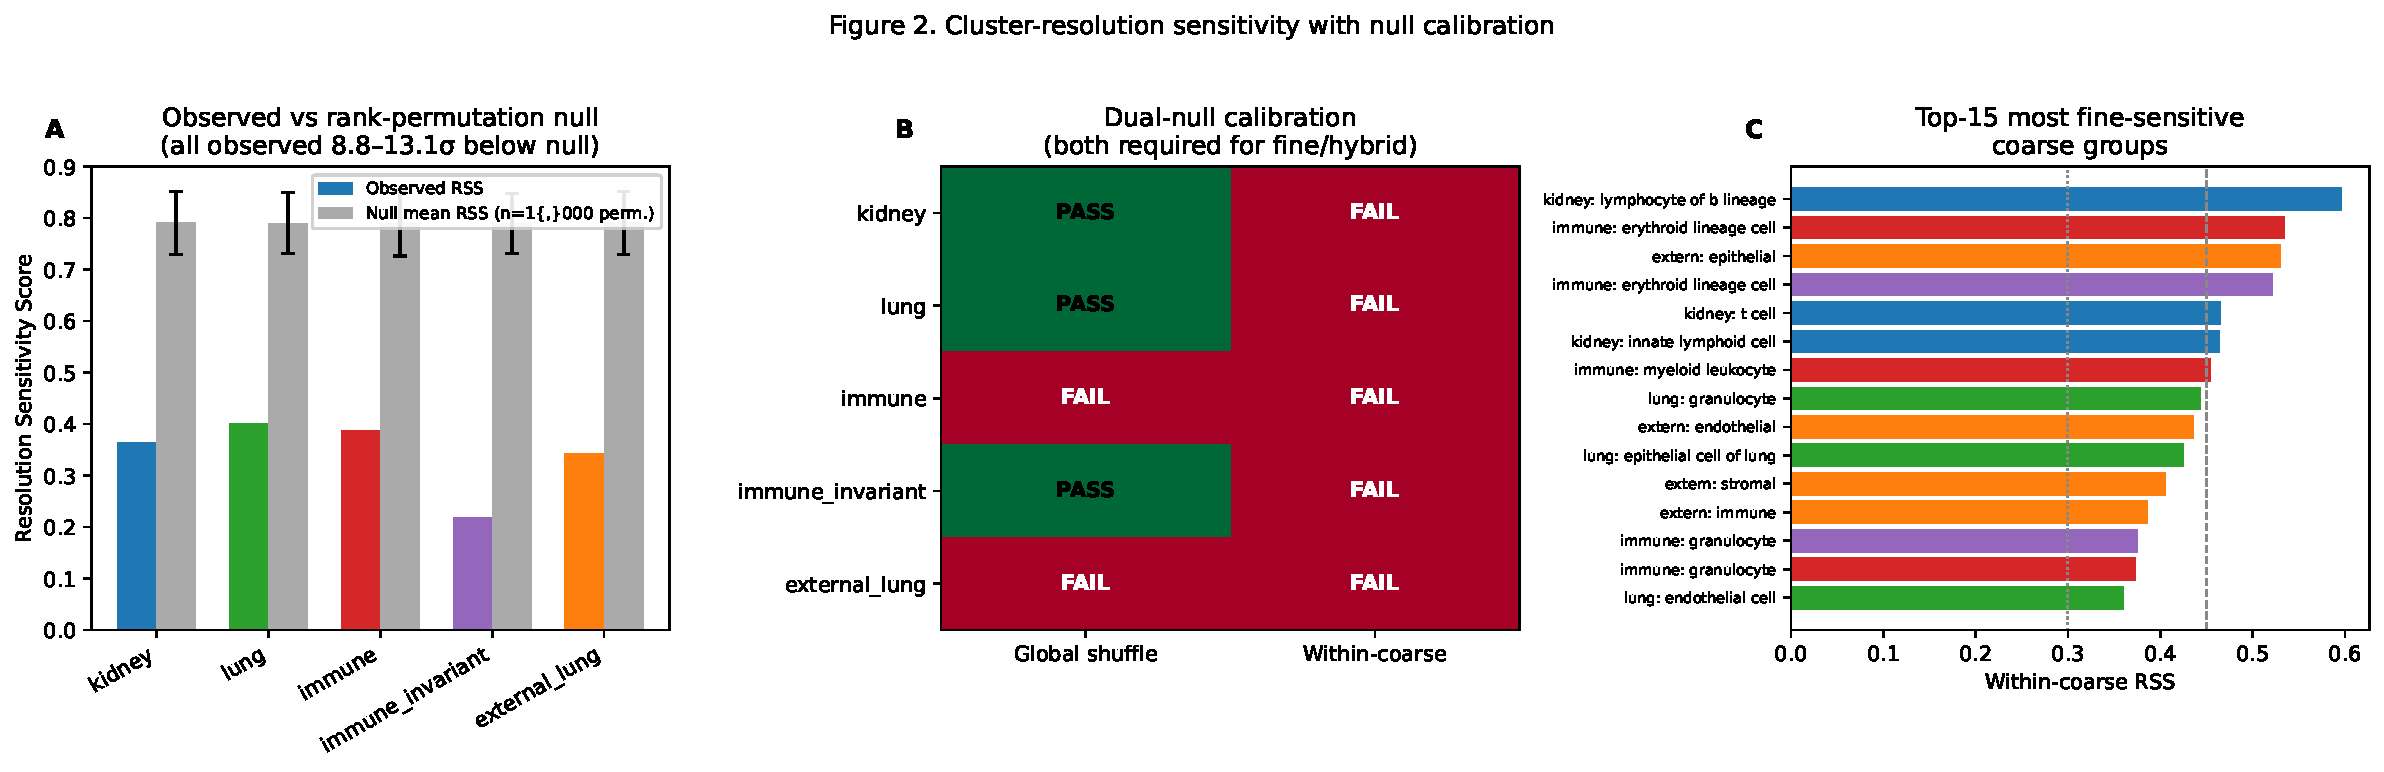
\includegraphics[width=\textwidth,height=0.82\textheight,keepaspectratio]{figures/fig2_resolution.pdf}
\caption{\textbf{Cluster-resolution sensitivity and dual-null calibration.}
(A)~Resolution Sensitivity Score across five cohorts with base recommendation thresholds.
(B)~Dual-null calibration results: global-shuffle and within-coarse constrained-shuffle
pass/fail for each cohort, with final calibrated recommendation.}
\label{fig:resolution}
\end{figure}

\subsection{Axis~3: Rare cell types exhibit a systematic reliability gap}

Across 88 cell types in four datasets, rare types were not significantly worse on
global rank stability (Spearman: rare 0.884 vs.\ abundant 0.851, $p = 0.835$) but
were significantly worse on decision-level metrics: top-$k$ Jaccard (0.625 vs.\ 0.731,
$p = 4.1 \times 10^{-3}$), null-separation AUC (0.520 vs.\ 0.620,
$p = 5.3 \times 10^{-8}$), and null-tail gap ($-0.062$ vs.\ 0.082,
$p = 1.5 \times 10^{-7}$). The reliability gate was passed by 0/22 rare cell types
and 4/22 abundant cell types (Figure~\ref{fig:rare}A--B).

Under the conservative dual-null (minimum AUC across cell-permutation and gene-shuffle
models), the rare--abundant gap attenuated but remained significant
(AUC gap 0.018, $p = 6.8 \times 10^{-4}$; tail gap 0.037, $p = 0.015$). Shared-panel
sensitivity analysis showed heterogeneous agreement with adaptive-panel results
(dataset Spearman 0.09--0.93 for null-AUC ordering): strong in immune and kidney
but weak in lung, indicating that the rare-type deficit is partially but not fully
explained by panel-construction choices.

Minimum reliable cell-size estimates ranged from 287 (external lung, model-based) to
16{,}486 (lung, empirical reliable minimum), underscoring that some tissues require
very large cell-type samples before mechanistic edges reach reliability thresholds.

\begin{figure}[ht]
\centering
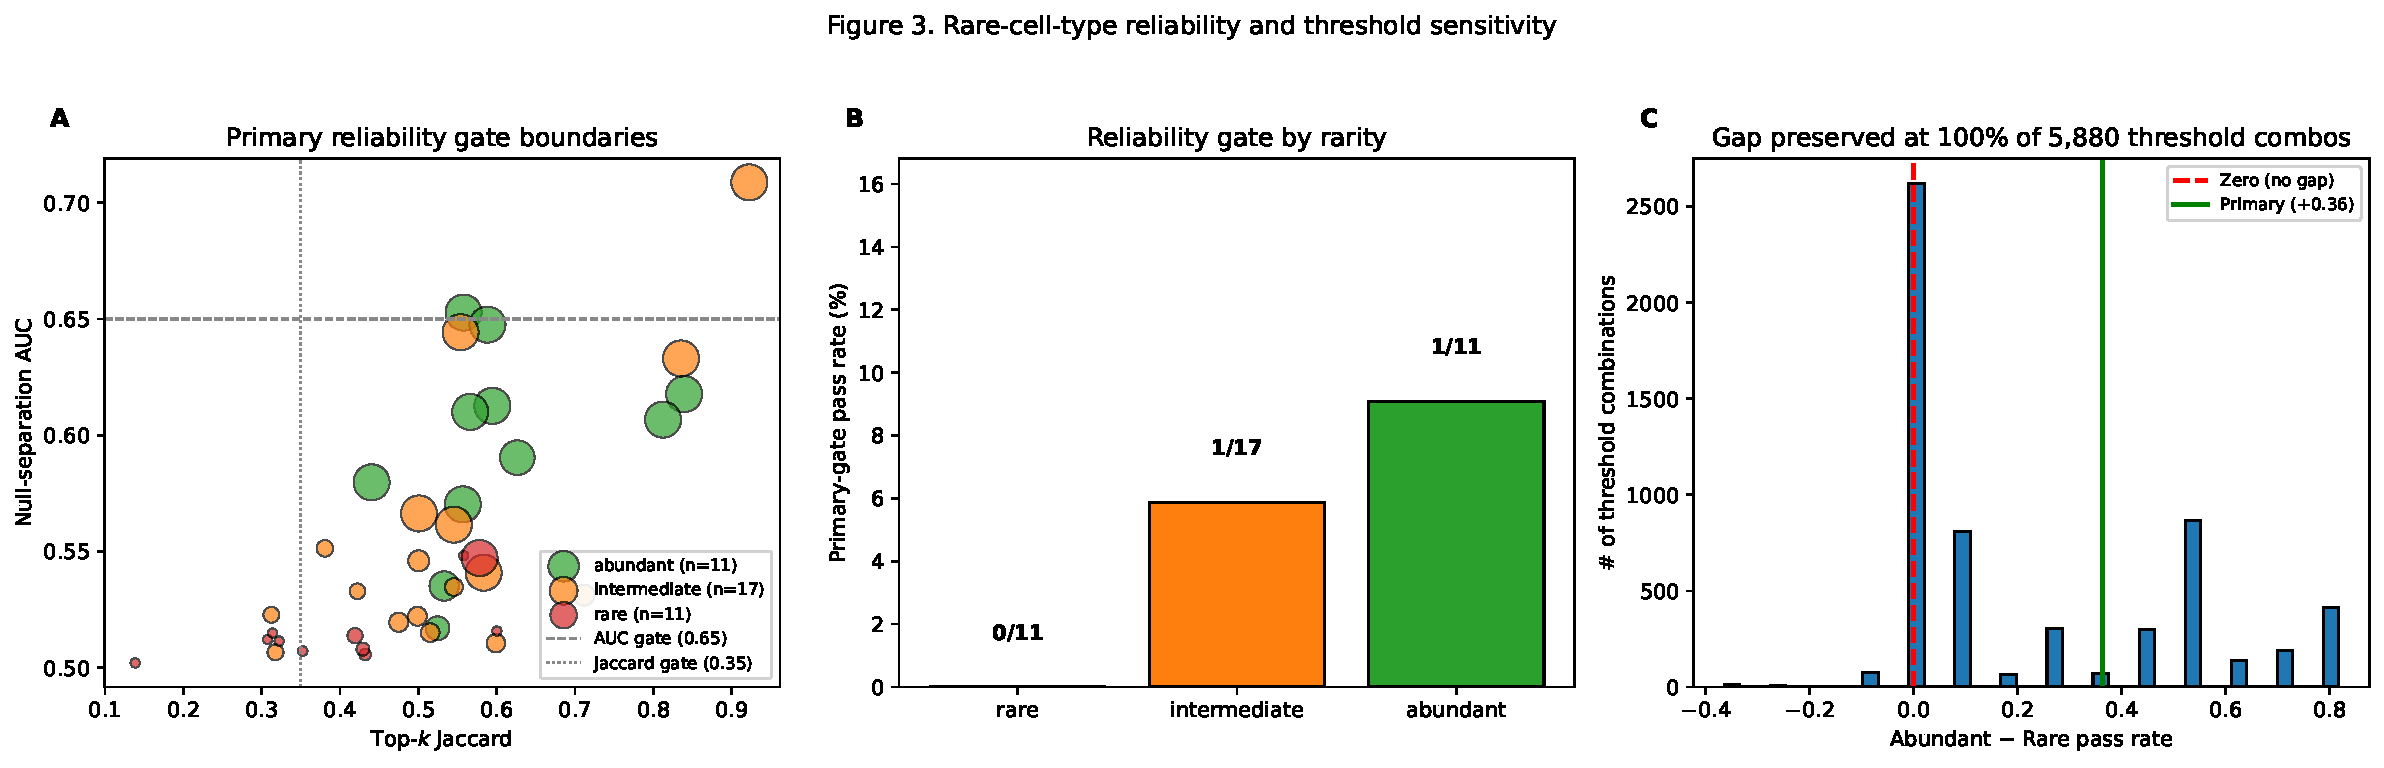
\includegraphics[width=\textwidth,height=0.82\textheight,keepaspectratio]{figures/fig3_rare.pdf}
\caption{\textbf{Rare-cell-type reliability stress test.}
(A)~Null-separation AUC and top-$k$ Jaccard as functions of cell count, colored by
rarity group. (B)~Reliability-gate pass rates: 0\% rare versus 18\% abundant.
(C)~Minimum reliable cell-size estimates by dataset.}
\label{fig:rare}
\end{figure}

\subsection{Axis~4: Donor generalization requires 6--8 donors and is partly composition-mediated}

Under the corrected fixed-holdout protocol, immune-tissue transfer improved monotonically
from train$= 2$ to train$= 10$ donors (Spearman 0.568 $\to$ 0.683; top-100 overlap
0.445 $\to$ 0.540), eliminating the apparent interior optimum from the initial
complementary-split protocol (Figure~\ref{fig:donor}A). The baseline complementary-split
design had inflated transfer estimates by a mean of $+0.080$ Spearman and $+0.102$
top-100 overlap at shared train counts.

Expanding to top-20 donors (including long-tail low-count donors) lowered all transfer
metrics (train$= 16$: Spearman 0.627, overlap@100 0.460), indicating that top-donor-only
evaluation was optimistic for broad-cohort deployment. Updated recommendation using a
90\%-of-best criterion is \textbf{6 train donors}; the 95\%-of-best conservative
criterion yields \textbf{8 train donors} (Figure~\ref{fig:donor}B).

Composition-matched controls (top-8 donors, 3 shared broad classes, 62 cells/donor)
reduced transfer estimates by 16.3\% (Spearman: 0.707 $\to$ 0.591) and 10.7\%
(overlap@100: 0.610 $\to$ 0.545), confirming that cell-type composition explains a
substantial but incomplete fraction of apparent donor generalization. Above-null signal
remained robust even under the strictest protocol (lift@100, defined as observed
overlap at rank 100 divided by chance expectation: 37.8--44.3$\times$).

\begin{figure}[ht]
\centering
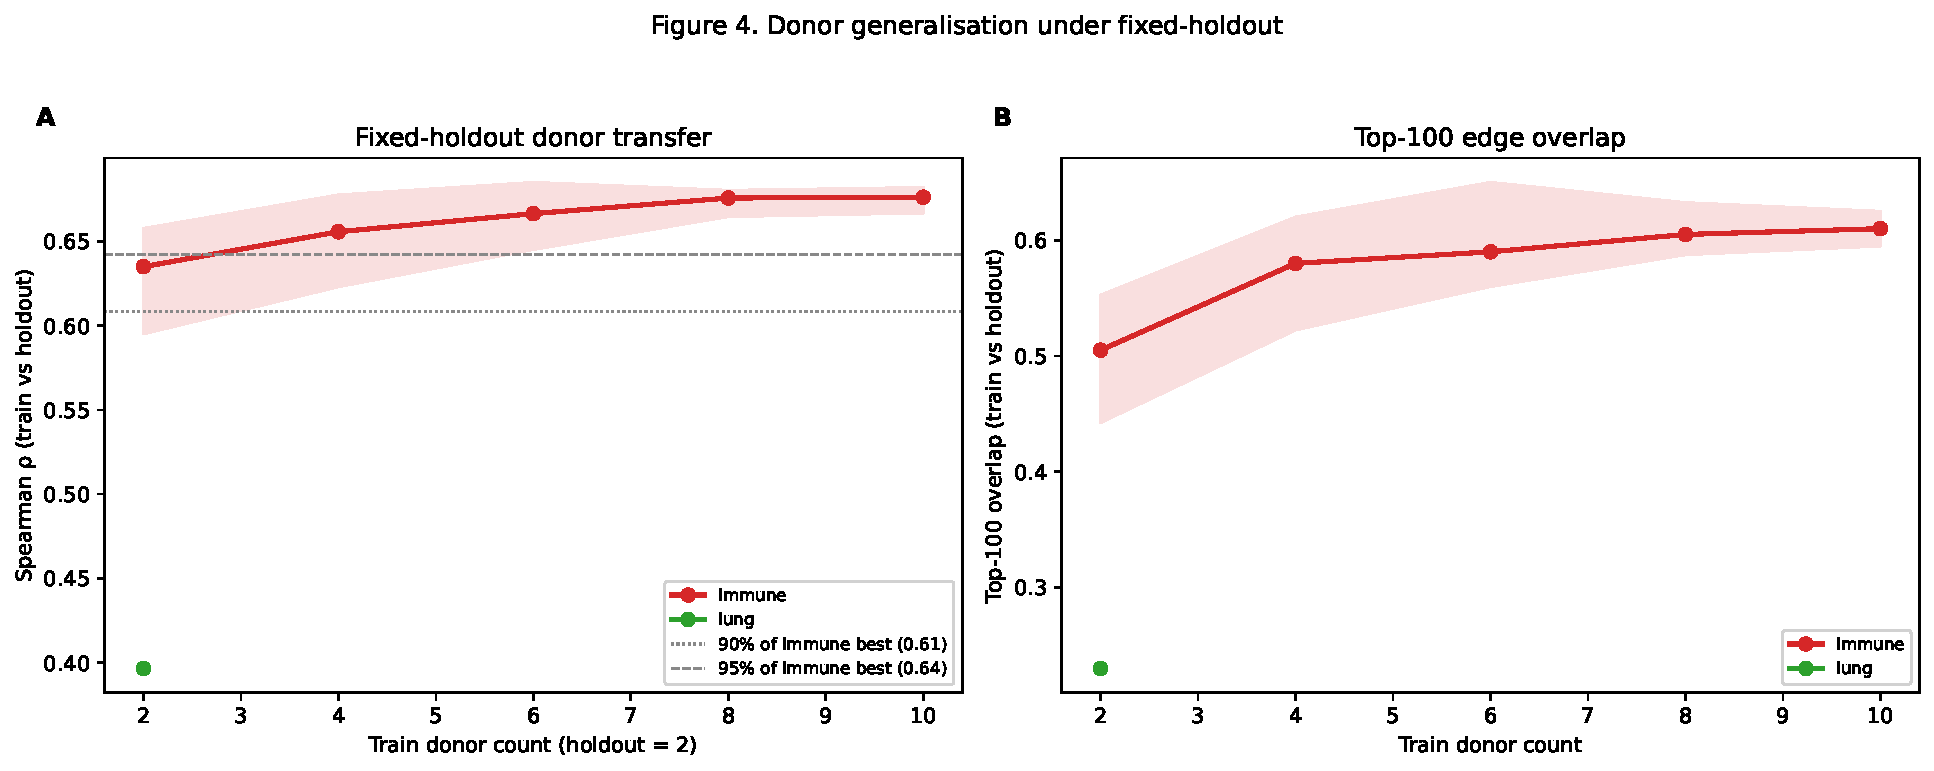
\includegraphics[width=\textwidth]{figures/fig4_donor.pdf}
\caption{\textbf{Donor generalization under fixed-holdout and composition control.}
(A)~Immune transfer curves under fixed-holdout (holdout$= 2$) for top-12 and top-20
donor panels. (B)~Composition-matched versus unmatched transfer in the top-8 panel.
Error bands show interquartile range over 30--40 sampled splits.}
\label{fig:donor}
\end{figure}

\subsection{Axis~5: Integration reorders rankings substantially but does not improve perturbation-grounded validity}

Harmony integration produced moderate-to-large rank perturbations across all three
tissues: Spearman correlation with baseline ranged from 0.757 to 0.823, sign-flip
rates from 8.1\% to 12.7\%, and top-500 overlap from 0.552 to 0.688
(Figure~\ref{fig:integration}A). Bootstrap confidence intervals confirmed stable
effect sizes.

Curated-reference precision@500 showed nominal DoRothEA/TRRUST gains in immune and
kidney, but after paired swap-based significance testing with BH-FDR correction,
robust gains were concentrated in TRRUST only (immune and kidney: $\Delta$ precision
+0.026 to +0.028, FDR $< 0.05$; Figure~\ref{fig:integration}B). DoRothEA and
ChIP-seq-backed gains were not FDR-significant. Perturbation validation using external
Dixit-derived tables showed no significant Harmony improvement: top-500 perturbation
swap deltas were small and negative ($-0.002$ to $-0.004$; FDR $= 1.0$).

A hyperparameter sweep over $n_{\text{pcs}} \in \{30, 50, 80\}$ revealed a
robustness--performance tradeoff: top-500 overlap increased monotonically with PCs
(immune: 0.590 $\to$ 0.736), while DoRothEA precision peaked at intermediate PCs
and declined at higher dimensionality.

\begin{figure}[ht]
\centering
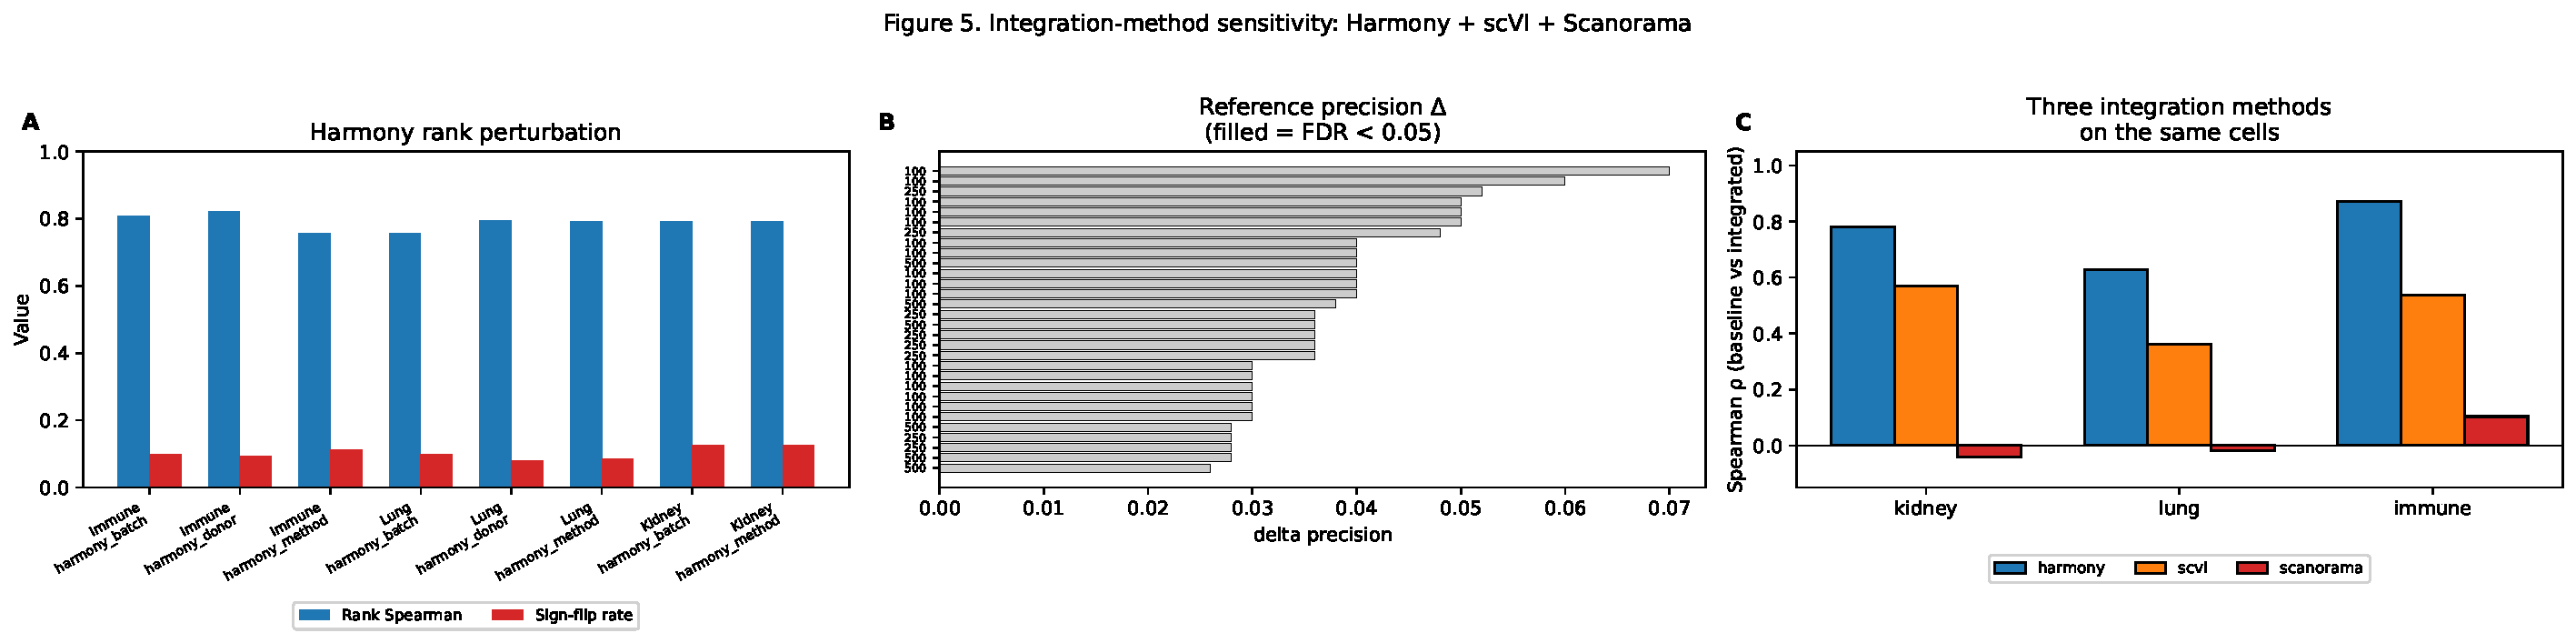
\includegraphics[width=\textwidth,height=0.82\textheight,keepaspectratio]{figures/fig5_integration.pdf}
\caption{\textbf{Integration-method sensitivity.}
(A)~Rank Spearman and top-500 overlap for Harmony variants across three tissues.
(B)~Reference precision@500 deltas with paired swap significance; filled bars indicate
FDR $< 0.05$. (C)~Harmony hyperparameter sweep: overlap versus DoRothEA precision
as a function of $n_{\text{pcs}}$.}
\label{fig:integration}
\end{figure}

\subsection{Cross-axis fragility synthesis}

Table~\ref{tab:fragility} summarizes the fragility profile across all five axes and
datasets, and Figure~\ref{fig:crossaxis} visualizes the per-axis pass/marginal/fail
status for each dataset. Several cross-axis interactions emerge:

\begin{itemize}
\item \textbf{Cell count constrains rare-type power}: the MVCC of $>$3{,}000 cells
      for unconstrained inference implies that most rare cell types (typically $< 500$
      cells) are inherently underpowered, consistent with the 0\% reliability-gate
      passage observed in Axis~3.
\item \textbf{Resolution choice modulates donor transfer}: coarse clustering pools
      cell-type variation that would otherwise require per-donor composition matching,
      partially explaining why coarse-level recommendations are more robust.
\item \textbf{Integration rotates shared covariance geometry}: Harmony's rank
      perturbation affects the correlation structure on which cell-count stability,
      resolution sensitivity, and rare-type null separation all depend.
\item \textbf{No axis is universally benign}: every dataset fails at least two axes
      by their respective calibrated criteria, and no single corrective (more cells,
      coarser clustering, more donors, integration) resolves all fragilities simultaneously.
\end{itemize}

\begin{figure}[ht]
\centering
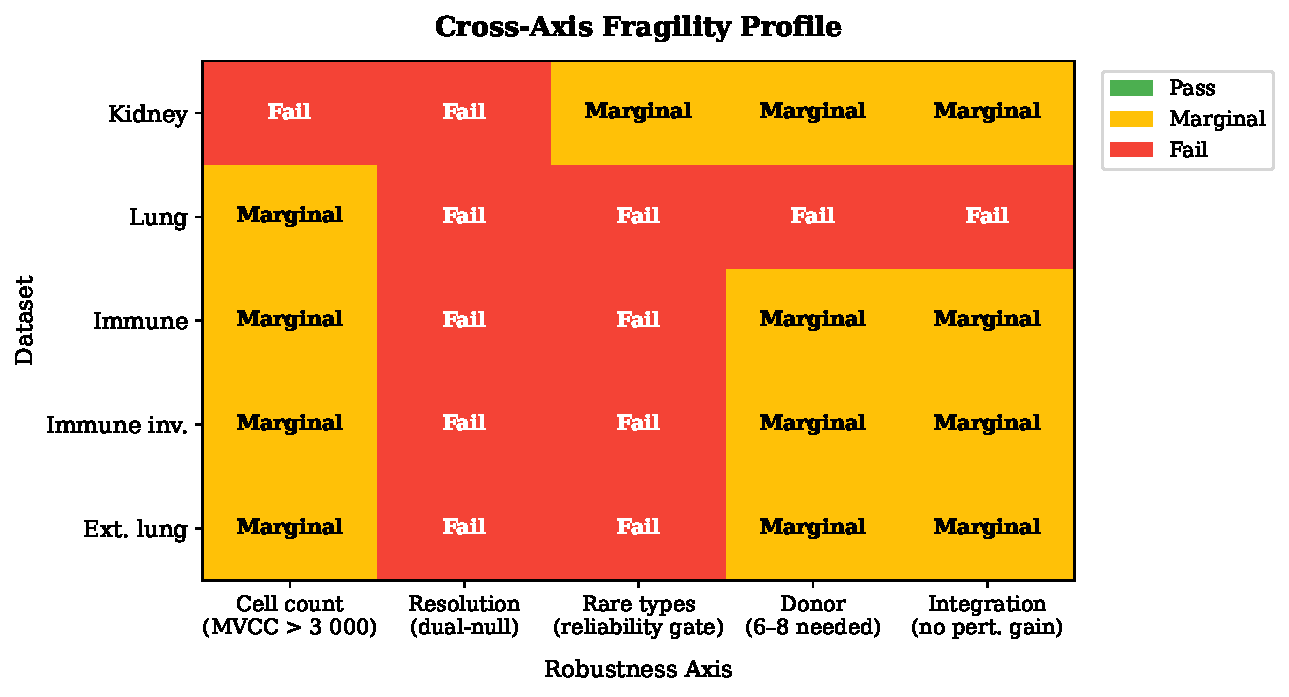
\includegraphics[width=0.85\textwidth]{figures/fig6_cross_axis.pdf}
\caption{\textbf{Cross-axis fragility summary.}
Heatmap showing pass (green), marginal (yellow), and fail (red) status for each
axis--dataset combination under calibrated criteria.}
\label{fig:crossaxis}
\end{figure}

\begin{table}[ht]
\centering
\caption{Per-axis robustness summary with key metric, calibrated threshold, and practical recommendation.}
\label{tab:fragility}
\small
\begin{tabularx}{\textwidth}{lXlX}
\toprule
\textbf{Axis} & \textbf{Key Metric} & \textbf{Threshold} & \textbf{Recommendation} \\
\midrule
Cell count & MVCC (top-1k Jaccard $>$ 0.5) & $>$3{,}000 cells &
  Use $\geq$3{,}000 cells or apply prior constraints \\
\addlinespace
Resolution & Dual-null pass rate & Both nulls must pass &
  Default to coarse; report within-class heterogeneity \\
\addlinespace
Rare types & Reliability gate (5 criteria) & All must pass &
  Treat rare-cell edges as hypothesis-generating only \\
\addlinespace
Donor & Fixed-holdout Spearman & 90\% of best & Collect $\geq$6 donors (8 conservative) \\
\addlinespace
Integration & Perturbation swap $\Delta$ & FDR $<$ 0.05 &
  Report multi-reference validation; avoid universal claims \\
\bottomrule
\end{tabularx}
\end{table}

% ============================================================
% 4. DISCUSSION
% ============================================================
\section{Discussion}

This audit demonstrates that GRN edge rankings from single-cell data are fragile
along multiple axes simultaneously, and that apparent robustness along one axis
(e.g., coarse rank stability for rare types) can mask failure along another
(e.g., null separation). The adversarial-review methodology that we applied to
each axis is itself a contribution: by requiring corrective experiments before
claims are updated, it systematically closes the gap between initial findings and
defensible conclusions.

\paragraph{Practical implications.}
Table~\ref{tab:guidelines} provides concrete guidance for practitioners.
The central message is that no single parameter choice can guarantee robust GRN
inference; instead, robustness must be demonstrated along each relevant axis for
the specific tissue, cell count, and analytical choices at hand.

\begin{table}[ht]
\centering
\caption{Practical guidelines for robust GRN inference from single-cell data.}
\label{tab:guidelines}
\small
\begin{tabularx}{\textwidth}{lX}
\toprule
\textbf{Decision Point} & \textbf{Guideline} \\
\midrule
\textit{Sample size} &
  Target $\geq$3{,}000 cells for unconstrained inference, or use informative prior
  constraints (DoRothEA/TRRUST) which stabilize rankings at 200+ cells. \\
\addlinespace
\textit{Clustering} &
  Default to coarse clustering unless dual-null calibration (global + within-coarse
  constrained shuffle) confirms that fine resolution adds separable signal. Report
  within-class RSS for compartment-level uncertainty. \\
\addlinespace
\textit{Rare cell types} &
  Report null-separation AUC alongside stability for every cell type. Flag rare types
  ($< 250$ cells) as hypothesis-generating. Provide minimum-reliable-size estimates
  with uncertainty status. \\
\addlinespace
\textit{Donor coverage} &
  Collect $\geq$6 donors (8 for conservative generalization). Use fixed-holdout
  evaluation, not complementary splits. Report composition-controlled transfer alongside
  raw transfer. \\
\addlinespace
\textit{Integration} &
  Report at least paired swap significance for reference gains, plus one
  perturbation-backed metric when available. Include hyperparameter sensitivity
  ($n_{\text{pcs}}$). Avoid universal claims of biological improvement. \\
\addlinespace
\textit{Cross-axis audit} &
  Report a fragility profile (Table~\ref{tab:fragility}) covering all axes relevant to
  the study design. Acknowledge which axes were not testable and why. \\
\bottomrule
\end{tabularx}
\end{table}

\paragraph{Comparison to existing benchmarks.}
Published GRN benchmarks~\citep{Pratapa2020, Chen2023} have focused primarily on
accuracy relative to gold-standard references, treating preprocessing as fixed.
Our audit complements these by asking whether rankings are \emph{stable} across
realistic analytical perturbations, a necessary condition for practical utility.
The two perspectives are not redundant: a method can be accurate under one
configuration and fragile under perturbation, or robustly mediocre across all
configurations.

\paragraph{Limitations.}
Several limitations apply across the audit. First, all edge scoring is
correlation-based and does not directly estimate causal regulatory effects;
although correlation on normalized counts avoids zero-inflation
artifacts~\citep{Svensson2020}, it remains susceptible to confounding by
shared upstream regulators~\citep{Kharchenko2014}.
Second, the audit covers Tabula Sapiens tissues and one external lung cohort;
generalization to disease tissues, developmental atlases, or cross-species
comparisons remains untested. Third, adversarial null designs (particularly
constrained shuffles) may be overly strict for certain scoring families,
potentially leading to conservative recommendations that reject genuine fine-scale
signal. Fourth, perturbation-backed validation data remain sparse, limiting
statistical power for perturbation swap tests. Fifth, we evaluated only
Harmony among integration methods; broader comparisons including scVI and
Scanorama~\citep{Gayoso2022, Hie2019}, guided by recent integration
benchmarks~\citep{Luecken2022, Tran2020}, are warranted.

% ============================================================
% 5. CONCLUSION
% ============================================================
\section{Conclusion}

We present the first systematic multi-axis robustness audit of GRN inference from
single-cell transcriptomics, spanning cell count, clustering resolution, rare-cell
reliability, donor generalization, and integration-method sensitivity. The audit
reveals that fragility is pervasive, axis-specific, and interactive: no dataset
passed all five axes under calibrated criteria, and corrective measures along one
axis do not automatically resolve others. We provide a practical guidelines table
and an open-source framework, consisting of modular Python scripts for each axis
(subsampling sweeps, resolution calibration with dual nulls, rare-type reliability
gates, donor-holdout curves, and integration swap tests), that enables practitioners
to conduct analogous audits for their own datasets and inference pipelines before
publishing GRN claims.

% ============================================================
% AUTHOR CONTRIBUTIONS
% ============================================================
\section*{Author Contributions}

I.K.\ conceived the study, designed the five-axis robustness audit framework,
implemented all computational pipelines, performed all statistical analyses,
generated all figures and tables, and wrote the manuscript.

% ============================================================
% FUNDING
% ============================================================
\section*{Funding}

This research received no specific grant from any funding agency in the public,
commercial, or not-for-profit sectors.

% ============================================================
% CONFLICT OF INTEREST
% ============================================================
\section*{Conflict of Interest}

None declared.

% ============================================================
% DATA AND CODE AVAILABILITY
% ============================================================
\section*{Data and Code Availability}

All source code, result data, and figure-generation scripts are publicly
available at \url{https://github.com/Biodyn-AI/grn-robustness-audit}.
The repository is self-contained: running \texttt{make all} regenerates all
figure panels from the included CSV result files, composes the six composite
PDF figures, and compiles this manuscript. Per-axis result CSVs are provided
in \texttt{data/} and individual figure panels in \texttt{source\_panels/};
see the repository README for a full data dictionary and step-by-step
reproduction instructions.
Raw single-cell data are from the Tabula Sapiens Consortium and are available at
\url{https://tabula-sapiens-portal.ds.czbiohub.org/}.

% ============================================================
% SUPPLEMENTARY INFORMATION
% ============================================================
\section*{Supplementary Information}

Supplementary tables with per-dataset, per-axis detailed metrics and the full
hyperparameter-grid results are available in the GitHub repository.

% ============================================================
% ABBREVIATIONS
% ============================================================
\section*{Abbreviations}

\noindent
AUC: Area Under the Curve;
BH: Benjamini--Hochberg;
FDR: False Discovery Rate;
GRN: Gene Regulatory Network;
MVCC: Minimum Valid Cell Count;
PCA: Principal Component Analysis;
RSS: Resolution Sensitivity Score;
scRNA-seq: Single-Cell RNA Sequencing;
TF: Transcription Factor.

% ============================================================
% REFERENCES
% ============================================================
\begin{thebibliography}{99}

\bibitem[Aibar et~al., 2017]{Aibar2017}
Aibar, S., Gonz{\'a}lez-Blas, C.~B., Moerman, T., et~al. (2017).
\newblock SCENIC: single-cell regulatory network inference and clustering.
\newblock \textit{Nature Methods}, 14(11):1083--1086.

\bibitem[Chen and Mar, 2018]{Chen2023}
Chen, S. and Mar, J.~C. (2018).
\newblock Evaluating methods of inferring gene regulatory networks highlights their
  lack of performance for single cell gene expression data.
\newblock \textit{BMC Bioinformatics}, 19(1):232.

\bibitem[Cui et~al., 2024]{Cui2024}
Cui, H., Wang, C., Maan, H., et~al. (2024).
\newblock scGPT: toward building a foundation model for single-cell multi-omics
  using generative AI.
\newblock \textit{Nature Methods}, 21(8):1470--1480.

\bibitem[Dixit et~al., 2016]{Dixit2016}
Dixit, A., Parnas, O., Li, B., et~al. (2016).
\newblock Perturb-Seq: Dissecting molecular circuits with scalable single-cell RNA
  profiling of pooled genetic screens.
\newblock \textit{Cell}, 167(7):1853--1866.

\bibitem[Garcia-Alonso et~al., 2019]{GarciaAlonso2019}
Garcia-Alonso, L., Holland, C.~H., Ibrahim, M.~M., Turei, D., and
  Saez-Rodriguez, J. (2019).
\newblock Benchmark and integration of resources for the estimation of human
  transcription factor activities.
\newblock \textit{Genome Research}, 29(8):1363--1375.

\bibitem[Gayoso et~al., 2022]{Gayoso2022}
Gayoso, A., Lopez, R., Xing, G., et~al. (2022).
\newblock A Python library for probabilistic analysis of single-cell omics data.
\newblock \textit{Nature Biotechnology}, 40(2):163--166.

\bibitem[Han et~al., 2018]{Han2018}
Han, H., Cho, J.-W., Lee, S., et~al. (2018).
\newblock TRRUST v2: an expanded reference database of human and mouse
  transcriptional regulatory interactions.
\newblock \textit{Nucleic Acids Research}, 46(D1):D199--D202.

\bibitem[Hie et~al., 2019]{Hie2019}
Hie, B., Bryson, B., and Berger, B. (2019).
\newblock Efficient integration of heterogeneous single-cell transcriptomes using
  Scanorama.
\newblock \textit{Nature Biotechnology}, 37(6):685--691.

\bibitem[Kharchenko et~al., 2014]{Kharchenko2014}
Kharchenko, P.~V., Silberstein, L., and Scadden, D.~T. (2014).
\newblock Bayesian approach to single-cell differential expression analysis.
\newblock \textit{Nature Methods}, 11(7):740--742.

\bibitem[Korsunsky et~al., 2019]{Korsunsky2019}
Korsunsky, I., Millard, N., Fan, J., et~al. (2019).
\newblock Fast, sensitive and accurate integration of single-cell data with
  Harmony.
\newblock \textit{Nature Methods}, 16(12):1289--1296.

\bibitem[Luecken and Theis, 2019]{Luecken2019}
Luecken, M.~D. and Theis, F.~J. (2019).
\newblock Current best practices in single-cell RNA-seq analysis: a tutorial.
\newblock \textit{Molecular Systems Biology}, 15(6):e8746.

\bibitem[Luecken et~al., 2022]{Luecken2022}
Luecken, M.~D., B{\"u}ttner, M., Chaichoompu, K., et~al. (2022).
\newblock Benchmarking atlas-level data integration in single-cell genomics.
\newblock \textit{Nature Methods}, 19(1):41--50.

\bibitem[Moerman et~al., 2019]{Moerman2019}
Moerman, T., Aibar Santos, S., Gonz{\'a}lez-Blas, C.~B., et~al. (2019).
\newblock GRNBoost2 and Arboreto: efficient and scalable inference of gene
  regulatory networks.
\newblock \textit{Bioinformatics}, 35(12):2159--2161.

\bibitem[Pratapa et~al., 2020]{Pratapa2020}
Pratapa, A., Jalihal, A.~P., Law, J.~N., Bharadwaj, A., and Murali, T.~M. (2020).
\newblock Benchmarking algorithms for gene regulatory network inference from
  single-cell transcriptomic data.
\newblock \textit{Nature Methods}, 17(2):147--154.

\bibitem[Svensson, 2020]{Svensson2020}
Svensson, V. (2020).
\newblock Droplet scRNA-seq is not zero-inflated.
\newblock \textit{Nature Biotechnology}, 38(2):147--150.

\bibitem[{The Tabula Sapiens Consortium}, 2022]{TabulaSapiens2022}
{The Tabula Sapiens Consortium}. (2022).
\newblock The Tabula Sapiens: A multiple-organ, single-cell transcriptomic atlas
  of humans.
\newblock \textit{Science}, 376(6594):eabl4896.

\bibitem[Tran et~al., 2020]{Tran2020}
Tran, H.~T.~N., Ang, K.~S., Chevrier, M., et~al. (2020).
\newblock A benchmark of batch-effect correction methods for single-cell RNA
  sequencing data.
\newblock \textit{Genome Biology}, 21(1):12.

\bibitem[Wolf et~al., 2018]{Wolf2018}
Wolf, F.~A., Angerer, P., and Theis, F.~J. (2018).
\newblock SCANPY: large-scale single-cell gene expression data analysis.
\newblock \textit{Genome Biology}, 19(1):15.

\end{thebibliography}

\end{document}
